%% -*- coding: utf-8 -*-
\documentclass[12pt,a4paper]{scrartcl} 
\usepackage[utf8]{inputenc}
\usepackage[english,russian]{babel}
\usepackage{indentfirst}
\usepackage{misccorr}
\usepackage{graphicx}
\usepackage{amsmath}
\begin{document}
\section{Введение}
\label{sec:intro}

% Что должно быть во введении
\begin{enumerate}
 \item Текстовая формулировка задачи
 \item Пример кода, решающего данную задачу
 \item Скриншот программы
\end{enumerate}
\section{Ход работы}
\label{sec:exp}
\subsection{Код приложения}
\label{sec:exp:code}
\begin{verbatim}
Кратчайшие пути на графе
#define _CRT_SECURE_NO_WARNINGS
#include <stdio.h>
#include <stdlib.h>
#define SIZE 6
int main()
{
  int a[SIZE][SIZE];
  int d[SIZE];
  int v[SIZE];
  int temp, minindex, min;
  int begin_index = 0;
  system("chcp 1251");
  system("cls");
  for (int i = 0; i<SIZE; i++)
  {
    a[i][i] = 0;
    for (int j = i + 1; j<SIZE; j++) {
      printf("Введите расстояние %d - %d: ", i + 1, j + 1);
      scanf("%d", &temp);
      a[i][j] = temp;
      a[j][i] = temp;
    }
  }
  for (int i = 0; i<SIZE; i++)
  {
    for (int j = 0; j<SIZE; j++)
      printf("%5d ", a[i][j]);
    printf("\n");
  }
  for (int i = 0; i<SIZE; i++)
  {
    d[i] = 10000;
    v[i] = 1;
  }
  d[begin_index] = 0;
  do {
    minindex = 10000;
    min = 10000;
    for (int i = 0; i<SIZE; i++)
    {
      if ((v[i] == 1) && (d[i]<min))
      {
        min = d[i];
        minindex = i;
      }
    }
    if (minindex != 10000)
    {
      for (int i = 0; i<SIZE; i++)
      {
        if (a[minindex][i] > 0)
        {
          temp = min + a[minindex][i];
          if (temp < d[i])
          {
            d[i] = temp;
          }
        }
      }
      v[minindex] = 0;
    }
  } while (minindex < 10000);
  printf("\nКратчайшие расстояния до вершин: \n");
  for (int i = 0; i<SIZE; i++)
    printf("%5d ", d[i]);

  int ver[SIZE]; 
  int end = 4; 
  ver[0] = end + 1;
  int k = 1; 
  int weight = d[end]; 

  while (end != begin_index)
  {
    for (int i = 0; i<SIZE; i++) 
      if (a[i][end] != 0)  
      {
        int temp = weight - a[i][end];
        if (temp == d[i]) 
        {
          weight = temp;
          end = i;       
          ver[k] = i + 1;
          k++;
        }
      }
  }
  printf("\nВывод кратчайшего пути\n");
  for (int i = k - 1; i >= 0; i--)
    printf("%3d ", ver[i]);
  getchar(); getchar();
  return 0;
}
\end{verbatim}
\subsection{формулы}
\label{sec:mathexample}

S[i]:=1; C[i]:=0
B[j]<=B[k]
Затем выполняются следующие операции:
S[j]:=1;
если B[k] > B[j]+A[j,k], то (B[k]:=B[j]+A[j,k]; C[k]:=j)
\newpage
\begin{document}
\section{Пример скриньшота программы }
Кратчайшие пути на графе
\label{sec:picexample}
\begin{figure}[h]
\centering
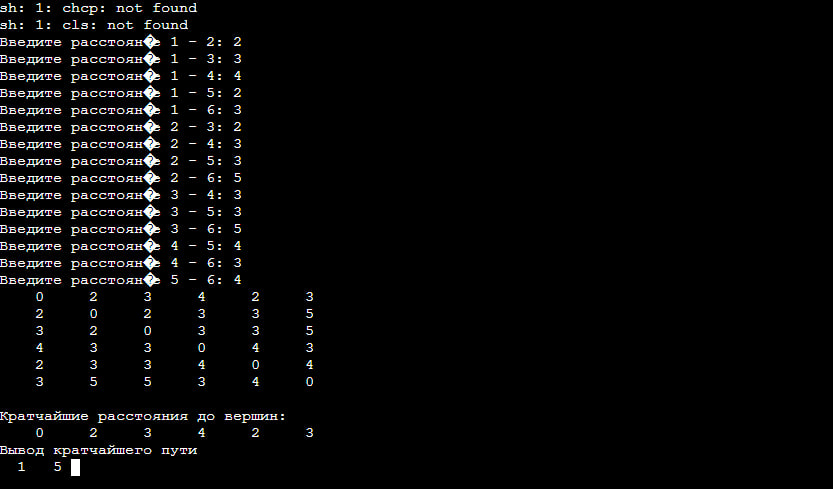
\includegraphics[scale=0.5]{скрин по с++ .png}
\caption{скриньшот программы}\label{fig:par}

\end{figure}
\newpage
\begin{document}
\label{sec:picexample}
\begin{figure}[h]
\centering
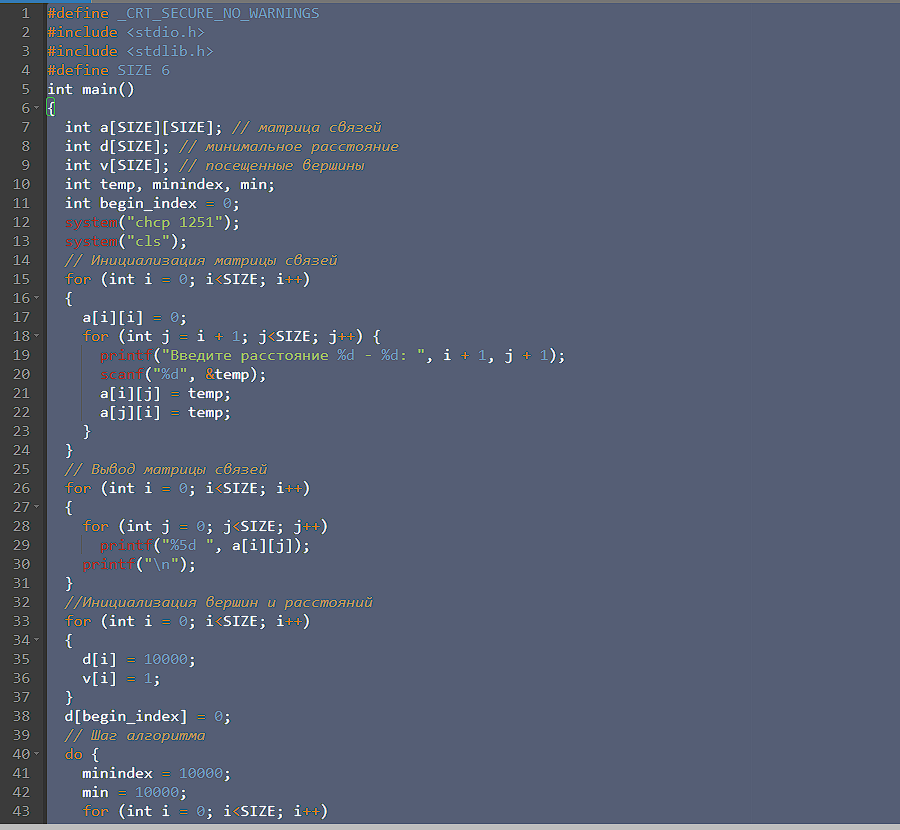
\includegraphics[scale=0.5]{скрин по с++ (2) .png}
\caption{скриньшот программы}\label{fig:par}


\end{figure}
\newpage
\begin{document}
\label{sec:picexample}
\begin{figure}[h]
\centering
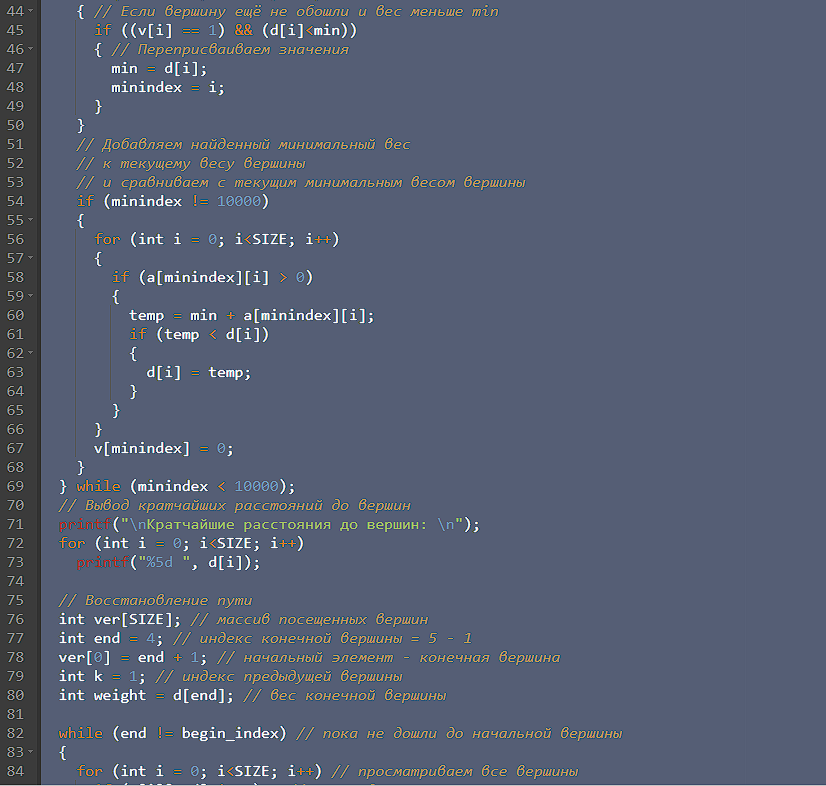
\includegraphics[scale=0.5]{скрин по с++ (3).png}
\caption{скриньшот программы}\label{fig:par}
\end{figure}

\newpage
\begin{document}
\label{sec:picexample}
\begin{figure}[h]
\centering
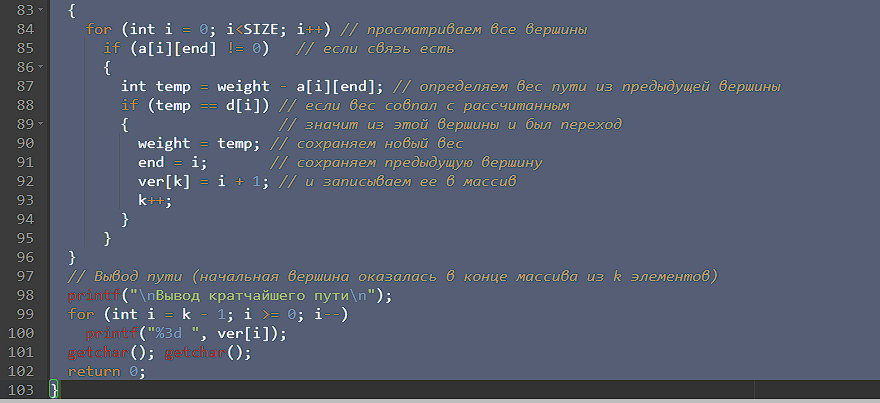
\includegraphics[scale=0.5]{скрин по с++ (4).png}
\caption{скриньшот программы}\label{fig:par}
\end{figure}

\section{ библиографические ссылки}

Для изучения «внутренностей» \TeX{} необходимо
изучить~\cite{Knuth-2003}, а для использования \LaTeX{} лучше
почитать~\cite{Lvovsky-2003, Voroncov-2005}.

\begin{thebibliography}{9}
\bibitem{Knuth-2003}Кнут Д.Э. Всё про \TeX. \newblock —- Москва: Изд. Вильямс, 2003 г. 550~с.
\bibitem{Lvovsky-2003}Львовский С.М. Набор и верстка в системе \LaTeX{}. \newblock —- 3-е издание, исправленное и дополненное, 2003 г.
\bibitem{Voroncov-2005}Воронцов К.В. \LaTeX{} в примерах. 2005 г.
\end{thebibliography}
\end{document}
\end{document}
\end{document}